\item \points{25} {\bf Linear regression: linear in what?}

In the first two lectures, you have seen how to fit a linear function of the data for the regression problem.  In this question, we will see how linear regression can be used to fit non-linear functions of the data using feature maps. We will also explore some of its limitations, for which future lectures will discuss fixes.

\begin{enumerate}
	\item \subquestionpoints{5} {\bf Learning degree-3 polynomials of the input}

Suppose we have a dataset $\{(x^{(i)}, y^{(i)})\}_{i=1}^{\nexp}$ where $x^{(i)}, y^{(i)} \in \mathbb{R}$. We would like to fit a third degree polynomial $h_{\theta}(x) = \theta_3x^3 + \theta_2x^2 + \theta_1x^1 + \theta_0$ to the dataset. The key observation here is that the function $h_{\theta}(x)$ is still linear in the unknown parameter $\theta$, even though it's not linear in the input $x$. This allows us to convert the problem into a linear regression problem as follows. 
	
	Let $\phi:\mathbb{R}\rightarrow \mathbb{R}^4$ be a function that transforms the original input $x$ to a $4$-dimensional vector defined as
	\begin{align}
	\phi(x) = \left[\begin{array}{c} 1\\ x \\ x^2 \\ x^3 \end{array}\right]\in \mathbb{R}^4 \label{eqn:feature}
	\end{align}
	Let $\hat{x}\in \mathbb{R}^4$ be a shorthand for $\phi(x)$, and let $\hat{x}^{(i)} \triangleq \phi(x^{(i)})$ be the transformed input in the training dataset. We construct a new dataset $\{(\phi(x^{(i)}), y^{(i)})\}_{i=1}^{\nexp} = \{(\hat{x}^{(i)}, y^{(i)})\}_{i=1}^{\nexp}$ by replacing the original inputs $x^{(i)}$'s by $\hat{x}^{(i)}$'s.  We see that fitting $h_{\theta}(x) = \theta_3x^3 + \theta_2x^2 + \theta_1x^1 + \theta_0$ to the old dataset is equivalent to fitting a linear function $h_{\theta}(\hat{x}) = \theta_3\hat{x}_3 +  \theta_2\hat{x}_2 + \theta_1\hat{x}_1 + \theta_0$ to the new dataset because 
	\begin{align}
	h_\theta(x) =  \theta_3x^3 + \theta_2x^2 + \theta_1x^1 + \theta_0 =  \theta_3 \phi(x)_3 + \theta_2\phi(x)_2 + \theta_1\phi(x)_1 + \theta_0 = \theta^T \hat{x}
	\end{align}
		
	In other words, we can use linear regression on the new dataset to find parameters $\theta_0,\dots, \theta_3$.

	Please write down 1) the objective function $J(\theta)$ of the linear regression problem on the new dataset $\{(\hat{x}^{(i)}, y^{(i)})\}_{i=1}^{\nexp}$ and 2) the update rule of the batch gradient descent algorithm for linear regression on the dataset $\{(\hat{x}^{(i)}, y^{(i)})\}_{i=1}^{\nexp}$. 
	
	\textit{Terminology:} 	In machine learning, $\phi$ is often called the feature map which maps the original input $x$ to a new set of variables. To distinguish between these two sets of variables, we will call $x$ the input {\bf attributes}, and call $\phi(x)$ the {\bf features}. (Unfortunately, different authors use different terms to describe these two things. In this course, we will do our best to follow the above convention consistently.)


        \ifnum\solutions=1 {
	  \begin{answer}
\newpage
\end{answer}

        }\fi

	\item \subquestionpoints{5} {\bf Coding question: degree-3 polynomial regression}


For this sub-question question, we will use the dataset provided in
the following files:
%
\begin{center}
	\url{src/featuremaps/{train,test}.csv}
\end{center}
%

Each file contains two columns: $x$ and $y$. In the terminology described in the introduction, $x$ is the attribute (in this case one dimensional) and $y$ is the output label.

Using the formulation of the previous sub-question, implement linear regression with \textbf{normal equations} using the feature map of degree-3 polynomials. Use the starter code provided in \texttt{src/featuremaps/featuremap.py} to implement the algorithm.

Create a scatter plot of the training data, and plot the learnt hypothesis as a smooth curve over it. Submit the plot in the writeup as the solution for this problem.

\emph{Remark: } Suppose $\widehat{X}$ is the design matrix of the transformed dataset. You may sometimes encounter a non-invertible matrix $\widehat{X}^T\widehat{X}$. For a numerically stable code implementation, always use \texttt{np.linalg.solve} to obtain the parameters directly, rather than explicitly calculating the inverse and then multiplying it with $\widehat{X}^Ty$.



        \ifnum\solutions=1 {
	  \begin{answer}
\begin{figure}[H]
    \centering
    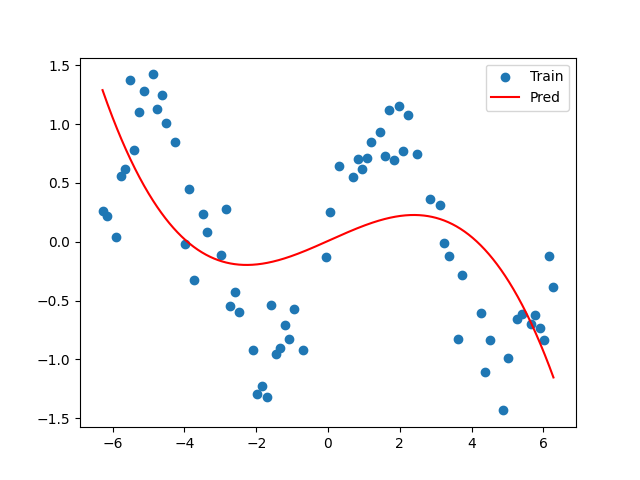
\includegraphics[width=9cm]{featuremaps/Prob_2_b.png}
\end{figure}
From the plot we observe that a 3rd degree polynomial does not seem to fit the data well.
\end{answer}

        }\fi

	\item \subquestionpoints{5} {\bf Coding question: degree-$k$ polynomial regression}

Now we extend the idea above to degree-$k$ polynomials by considering $\phi:\mathbb{R}\rightarrow \mathbb{R}^{k+1}$ to be 
\begin{align}
  \phi(x) = \left[\begin{array}{c} 1\\ x \\ x^2\\ \vdots \\x^k \end{array}\right]\in \mathbb{R}^{k+1} \label{eqn:feature-k}
\end{align}

Follow the same procedure as the previous sub-question, and implement the algorithm with $k=3,5,10,20$. Create a similar plot as in the previous sub-question, and include the hypothesis curves for each value of $k$ with a different color. Include a legend in the plot to indicate which color is for which value of $k$.

Submit the plot in the writeup as the solution for this sub-problem. Observe how the fitting of the training dataset changes as $k$ increases. Briefly comment on your observations in the plot.

        \ifnum\solutions=1 {
	  \begin{answer}
\begin{figure}[H]
    \centering
    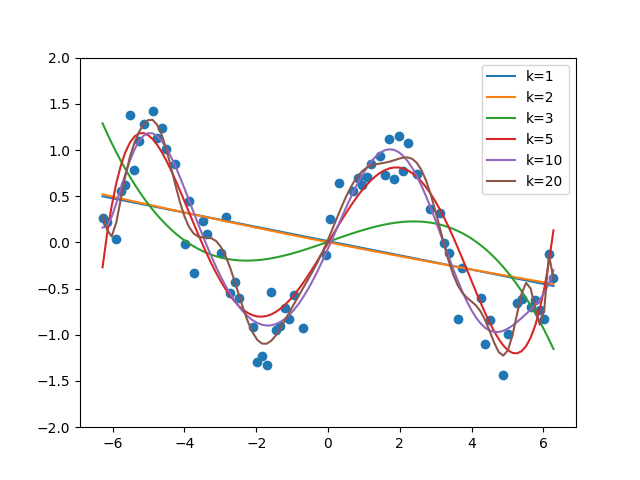
\includegraphics[width=9cm]{featuremaps/plot.png}
\end{figure}
From this plot we observe that higher degree polynomials fit the training data better. however if the axis were extended we would see how the polynomials of higher degree are very volatile and might not generalize well to other data.
\end{answer}

        }\fi

        \item \subquestionpoints{5} {\bf Coding question: other feature maps}

You may have observed that it requires a relatively high degree $k$ to fit the given training data, and this is because the dataset cannot be explained (i.e., approximated) very well by low-degree polynomials. By visualizing the data, you may have realized that $y$ can be approximated well by a sine wave. In fact, we generated the data by sampling from $y = \sin(x) + \xi$, where $\xi$ is noise with Gaussian distribution. Please update the feature map $\phi$ to include a sine transformation as follows:

\begin{align}
  \phi(x) = \left[\begin{array}{c} 1\\ x \\ x^2\\ \vdots \\x^k \\ \sin(x) \end{array}\right]\in \mathbb{R}^{k+2} \label{eqn:feature-sine}
\end{align}

With the updated feature map, train different models for values of $k=0,1,2,3,5,10,20$, and plot the resulting hypothesis curves over the data as before.

Submit the plot as a solution to this sub-problem. Compare the fitted models with the previous sub-question, and briefly comment about noticeable differences in the fit with this feature map.

        \ifnum\solutions=1 {
	  \begin{answer}
\begin{figure}[H]
    \centering
    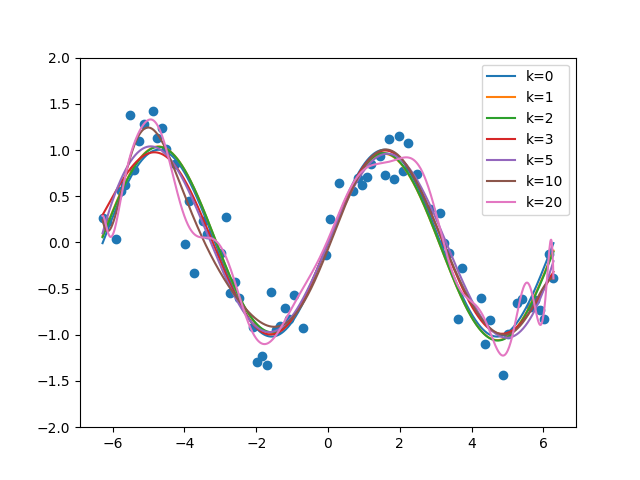
\includegraphics[width=9cm]{featuremaps/sine.png}
\end{figure}
Here we see that the polynomial terms seem to be redundant and that $sin(x)$ alone can model the data. The higher degree polynomial terms only contribute to overfitting.
\end{answer}

        }\fi

        \item \subquestionpoints{5} {\bf Overfitting with expressive models and small data}

For the rest of the problem, we will consider a small
dataset (a random subset of the dataset you have been using so far) with much fewer examples, provided in
the following file:
%
\begin{center}
	\url{src/featuremaps/small.csv}
\end{center}
%

We will be exploring what happens when the number of features start becoming bigger than the number of 
examples in the training set. Run your algorithm on this small dataset using the following feature map 
\begin{align}
\phi(x) = \left[\begin{array}{c} 1\\ x \\ x^2\\ \vdots \\x^k \end{array}\right]\in \mathbb{R}^{k+1} 
\end{align}
with $k = 1,2,5,10,20$. 

Create a plot of the various hypothesis curves (just like previous sub-questions). Observe how the fitting of the training dataset changes as $k$ increases. Submit the plot in the writeup and comment on what you observe.

        \ifnum\solutions=1 {
	  \begin{answer}
\begin{figure}[H]
    \centering
    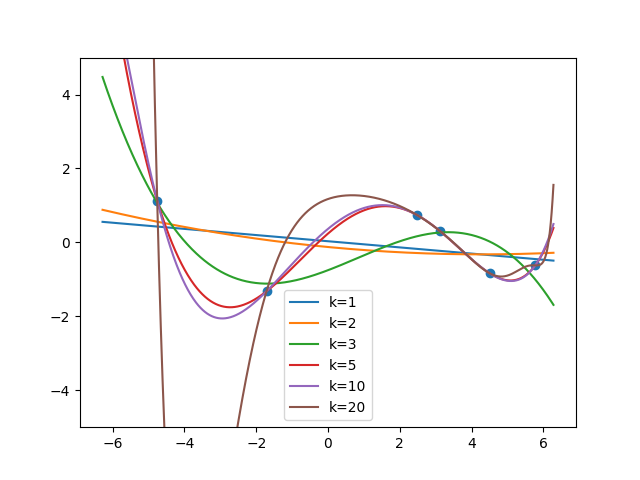
\includegraphics[width=9cm]{featuremaps/overfitting.png}
\end{figure}
For $n$ datapoints a polynomial of degree $n-1$ can perfectly interpolate the data. Therefore polynomials of degree $n-1$ can attain zero loss. There are 6 points in the data, and from the plot, we observe that the models with $k\ge 5$ fit the data perfectly.
\end{answer}

        }\fi
\end{enumerate}
